% chap3.tex (Definitions and Theorem)
\chapter{Methodology}
\section{Motivation }

We began by first making efforts to understand the influence of tree modeling as a data-adaptive approach on statistical inference and identify the source of overoptimism. The na\"{i}ve confidence interval (CI) estimates in (\ref{eqn-naive-ci}) involves two stochastic components $\bar{y}_t$ and $s_t$, the sample mean and sample standard deviation computed with observations in the training data $\mathcal{D}$ that fall into terminal node $t.$ In the following, we designed a study to investigate the performance of these two components in estimating the true node mean and node SD.

We generate training data $\mathcal{D}$ of size $n=500$ from one nonlinear model \citep{friedman1991multivariate}:
\begin{equation}
\label{met}
y \, = \,  -6 + 0.1 \exp(4x_1) + 4 \exp\{20(x_2 - 0.5)\} + 3 x_3 + 2 x_4 + x_5 + \varepsilon
\end{equation}
with $\varepsilon \sim \mathcal{N}(0, 1)$ and the $\mathbf{X_i}$'s are generated independently from random uniform[0,1] distribution of size $n = 500$.  A best-sized tree $\T$ is then constructed via pruning and cross-validation with the 1-SE rule \citep{breiman1984classification}. For each terminal node, $\bar{y}_t$ and $s_t$ are computed and recorded. Then we generate another independent test data set $\mathcal{D}'$ of size $n'=10,000.$ We send $\mathcal{D}'$ down to tree $ \T$ and recompute the node mean and SD $(\bar{y}'_t, s'_t)$.

\begin{figure}[H]
	\centering
	\includegraphics[scale=0.35, angle=270]{fig-inf.eps}
	\caption{Influence of tree modeling on inference: (a) node averages $\bar{y}_t$ and (b) node SD $s_t$ for $t \in \widetilde{T}$ computed with training data $\mathcal{D}$ and test data $\mathcal{D}'$. The green reference line is $y=x$. 
		\label{fig-inf-influence}}
\end{figure}
Figure \ref{fig-inf-influence} plots $\bar{y}_t$ vs.~$\bar{y}'_t$ in Panel (a) and $s_t$ vs.~$s'_t$ in Panel (b). It can be seen that $\bar{y}_t$ and~$\bar{y}'_t$ match well with each other, indicating the node averages can be used for prediction purposes. Nevertheless, $s_t$ from the training data $\mathcal{D}$ are generally smaller than $s'_t$ from the test data $\mathcal{D}'$, highlighting a systematic downward bias. Part of the reason accounting for the underestimated $s_t$ is that data is split with greedy search by minimizing the within-node impurity or variation when building up the tree model. Using $s_t$ directly would inevitably lead to inflated Type I error rates that hold accountable for the over-optimism. This observation in the $s_t$ bias distribution motivates us to correct the bias in the SD estimator $s_t$. 

\subsection{ Bias Correction Approach}
There are several techniques and approaches in dealing with bias correction. According to \cite{jiao2017bias} some general approaches to bias correction are the bootstrap, the jackknife, and the Taylor series. The jackknife uses a subsampling approach where the biases of estimators with different sample sizes are made to cancel each other while the bootstrap bias correction on the other hand uses the plug-in rule to estimate the bias. Taylor series is used to create an estimate (guess) of what a function or population parameter looks like through a derivative at a single point. However, the Taylor series according to \citep{jiao2017bias} is a less versatile method compared to the bootstrap and jackknife owning to its applicability to functions with specific global differentiability conditions. Given the natural grouping at each terminal node of decision trees, a small disturbance to the data set leads to different node membership observations. With this underlying behavior of trees and these methods discussed, bootstrapping \citep{tibshirani1993introduction} was chosen for our study. 

%One common method for bias correction is bootstrap  

\subsection{Bootstrapping}

The bootstrapping approach was introduced by \cite{efron19791977} among others with the motive of determining the variations in statistics when a theoretical variance is either unknown or not estimable and also correcting some forms of biasedness. The bootstrap methodology or concept is to simulate from an empirical distribution of a given data by means of resampling with replacement to obtain an approximation of the sampling distribution of the statistics. The bootstrap methodology estimates the sampling distribution of a given function $\Theta$ by recalculating its overall bootstrap samples $B_1, \ldots, B_n$ to obtain a set of bootstrapped statistics $\Theta_1, \Theta_2, \ldots, \Theta_B$, where $B$ is the number of bootstrap samples for a given set of data and a statistic of importance $\Theta$. The required approximate estimate can then be estimated by using $\Theta_1$, $\ldots$ , $\Theta_B$. The bias is obtained by taking the difference between the average of the bootstrapped statistics $\Theta_1$, $\ldots$, $\Theta_B$ and the given statistic $\Theta$. Let $\Theta_{b}$ represent the set of $\Theta_1, \Theta_2, \ldots, \Theta_B$, then;

\begin{equation}
\label{eqn-bias 1}
Bias\,=\, (\frac{1}{B} \sum_{b=1}^{B}\Theta_{b}) - \Theta
\end{equation}
Bias-corrected statistic is $\Theta^{c}$ now derived  as:
%\begin{equation}
$$\Theta^{c} = \Theta - Bias$$ 
$$  = 2\Theta - \, (\frac{1}{B} \sum_{b=1}^{B}\Theta_{b}) $$
%\end{equation}
Algorithm \ref{Alg-bootstrap} shows the iteration for a simple learning algorithm for a bootstrap-bias correction problem.

\vspace{.2in}
\IncMargin{1em}
\begin{algorithm}[H]
	\caption{Bootstrap Method} \label{Alg-bootstrap}
	\SetKwData{Left}{left}\SetKwData{This}{this}\SetKwData{Up}{up}
	\SetKwInOut{Input}{input}\SetKwInOut{Output}{output}
	\Input{data ${\X}_{i} \in \mathbb{R}^p ,\, size=n, \, \Theta$} 
	\Output{Acquire bias-corrected estimate $\Theta^{c}$}
	
	%\textbf{Take} $\X$  Data sample\;
	\Begin{
		\For{$1 \rightarrow b$  \KwTo $B$}{
			Derive ${\X}_{1}$,...,${\X}_{B}$ by resampling ${\X}_{i}$ with replacement. \newline
		Calculate $\Theta_{1}$, $\ldots$ , $\Theta_{B}$\\
			Estimate $\Theta^{c}$,\,with $\Theta_{1}$, $\ldots$ , $\Theta_{B}$ \newline
		}
		Acquire the bias-corrected estimate: \\  
		$\Theta^{c}$= 2$\Theta$ - $(\frac{1}{B} \sum_{b=1}^{B}\Theta_{b})$ , \,  where $\Theta_{b} \in (\Theta_{1}$, $\ldots$ , $\Theta_{B})$
	}
\end{algorithm}
\vspace{.2in}


\section{Exiting Methods}
\subsection{Bootstrap Calibration on  $\alpha$}
Given that scientists and investigators are often interested in making simultaneous inferences across all terminal nodes of $\T$, e.g., construct simultaneous confidence intervals for the node means. To deal with the multiplicity issue and over-optimism of tree modeling, \cite{loh2018subgroups} proposed using the bootstrap calibration (BC) approach \citep{loh1987calibrating, loh1991bootstrap} to tune the confidence level. Specifically, a constant $0 < \alpha' <1 $ is sought such that $(1-\alpha')$ intervals of the same form as (\ref{eqn-naive-ci}) has the $(1-\alpha)$ coverage for all terminal nodes. 
The BC algorithm in \cite{loh2018subgroups} was originally designed for tree-structured subgroup analysis (see, e.g., \citeauthor{su2009subgroup}, \citeyear{su2009subgroup}), where differential treatment effects are of the major concern. Applying the same procedure to ordinary regression trees leads to Algorithm \ref{Alg-BC}.

\vspace{.2in}
\IncMargin{1em}
\begin{algorithm}[H]
	\caption{Boostrap Calibration (BC)} \label{Alg-BC}
	\SetKwData{Left}{left}\SetKwData{This}{this}\SetKwData{Up}{up}
	\SetKwInOut{Input}{input}\SetKwInOut{Output}{output}
	\Input{data $\mathcal{D}=\{(\x_i, y_i) \in \mathbb{R}^p \times \mathbb{R}\}_{i=1}^n$ and $0 < \alpha_1 < \cdots < \alpha_K < \alpha < 1$ for a given $\alpha.$} 
	\Output{calibrated confidence coefficient $(1-\alpha').$}
	
	\textbf{initialize} $B$ -- \# bootstrap samples\;
	\Begin{
		Set coverage $\gamma_k = 0$ for $k =1, \ldots, K$ \;
		\For{$b \leftarrow 1$  \KwTo $B$}{
			draw a bootstrap sample $\mathcal{D}_b$ \;
			construct a best-sized tree $\mathcal{T}_b$ from $\mathcal{D}_b$ via pruning and cross validation\;
			summarize terminal nodes of $\mathcal{T}_b$ as $\{(n_t, \bar{y}_t, s_t): t \in \widetilde{\mathcal{T}}_b\}$ \; 
			send $\mathcal{D}$ down to $\mathcal{T}_b$ and recompute the mean response $\bar{y}'_t$ on basis of $\mathcal{D}$ %and record $n'_t$,% i.e., \# obs in node $t \cap \mathcal{D}$        
			\;
			
			set counters $c_k=0$ for $k =1, \ldots, K$ \;
			\For{$t \in \widetilde{\mathcal{T}}_b$}{
				\For{$k \leftarrow 1$  \KwTo $K$}{  
					construct $(1-\alpha_k) \times 100\%$ CI in node $t$: $(L_{tk}, U_{tk}) ~ \leftarrow ~ \bar{y}_t \pm z_{1-\alpha_k/2} \, \frac{\displaystyle s_t}{\displaystyle \sqrt{n_t}}$ , \If{$\bar{y}'_t \in (L_{tk}, U_{tk}),~ \forall t$}{$c_k := c_k  +1$\;} 
				}
			} 
			update $	\gamma_k := \gamma_k +  \frac{\displaystyle c_k}{\displaystyle | \widetilde{\mathcal{T}}_b |}$ and average $\gamma_k := \gamma_k/B$ for $k=1, \ldots, K$\;}
		
		find $k^\star \leftarrow$  smallest $k$ such that $\gamma_k < (1- \alpha)$, implying that $\gamma_{k^\star -1} \geq (1-\alpha)$ and 
		obtain $\alpha'$ via linear interpolation   $$ \alpha' ~=~  \alpha_{k^\star -1} + \frac{(1-\alpha) - \gamma_{k^\star}}{\gamma_{k^\star-1} - \gamma_{k^\star}} \, (\alpha_{k^\star} - \alpha_{k^\star-1}).$$  
	}
\end{algorithm}
%\vspace{.2in}
Now, given $\mathcal{D}$ as the data set and $\mathcal{D}_b$ to be a random bootstrap sample from $\mathcal{D}$. Let $\mathcal{T}_b$ be the set of all terminal nodes obtained from $\mathcal{D}_b$. For any $t \in \widetilde{\mathcal{T}}_b$, let $\bar{y}'_t$ be the node mean. We construct $(1-\alpha')$ confidence intervals for $\bar{y}'_t$ such that, the coverage probability of ($\mathcal{D}, \mathcal{D}_b, t, \alpha'$), averaged over the terminal nodes in the tree constructed from $\mathcal{D}_b$ has  expected value ($1-\alpha$).

Let $\gamma_k$ denote the set coverage that encompasses a terminal node of $\T$ of each observation in dataset $\mathcal{D}$, such that $P(\bar{y}'_t \in CI_{\gamma_k})$= ($1- \alpha$) $\forall$ $t\in \widetilde{\mathcal{T}}_b$, initializing $\gamma_k = 0$ for $k =1, \ldots, K$. We take $B$ bootstrap samples $\{ \mathcal{D}_b: b=1, \ldots, B\}.$ For each bootstrap sample $\mathcal{D}_b$, a best-sized tree $\T_b$ is constructed  via prunning and cross validation to obtain the estimates of $\mathcal{T}_b$ such as $\{(n_t, \bar{y}_t, s_t): t \in \widetilde{\mathcal{T}}_b\}$ \ for all terminal nodes of $\T_b.$ Sending $\mathcal{D}$ down to $\T_b$ and recomputing $\{ \bar{y}_t': t \in \widetilde{\mathcal{T}}_b\}$ \ for all terminal nodes of $\T_b.$ A counter coverage $c_{k}=0$ for $k =1, \ldots, K$ for each terminal node is set and we construct $(1-\alpha_k) \times 100\%$ CI in node $t$ for $\bar{y}_t$ based on set coverage $\alpha_k$ in Algorithm \ref{Alg-BC} . If $\bar{y}_t'$ $\in$ $(L_{tk}, U_{tk}) \in (\bar{y}_t' \pm z_{1-\alpha_k/2} \, \frac{\displaystyle s_t}{\displaystyle \sqrt{n_t}}$), then we update the set coverage {$c_k = c_k  +1$} for every mean node. We further update the $\gamma_k$ by averaging $c_k$ over the total number of trees and adding it to the initial coverage set $\gamma_k$ as outlined in line 18 of Algorithm \ref{Alg-BC}. Subsequently we average $\gamma_k$ over the number of bootstrap samples to obtain the smallest $K(k^\star)$, such that $\gamma_k < (1- \alpha)$, implying that $\gamma_{k^\star -1} \geq (1-\alpha)$. Now with  the  smallest $k$ and its corresponding $\gamma_k$ and $\alpha_k$ values our desired boostraped calibrated $\alpha'$ is obtained via linear interpolation. 



\section{Proposed  Method}
A statistically obtained prediction interval relies on the data $\mathcal{D}$. Making an reliable $(1-\alpha) \times 100\%$ confidence prediction base on the data relies on the stochastic estimates $\bar{y}_t$ and $s_t$ from the summary of decision tree output.  However, directly constructing this confidence interval with these estimates most especially the $s_t$ turns to be over-optimistic as shown in Figure \ref{fig-inf-influence}. Therefore we propose a method that keeps the $\alpha$ constant and corrects the downward biasedness in $s_t$ through bootstrapping to obtain a more honest unbiased estimate.

%It is therefore appropriate to resort to the boostrap bias correction (BBC) method to obtain a more honest  unbiased estimate of standard deviation ($s_t$) to arrive on an efficient  and consistent confident bound for predicting the node mean ($\bar{y}_t$) in decision trees.

\subsection{Bootstrap Bias Correction on $s_t$}

%\subsection{Correction on  SD}
In the bootstrap bias correction approach discussed, the estimates from bootstrap samples are compared to the original estimate and the averaged difference furnishes an estimator of the bias. However, there is one major obstacle with tree modeling. Trees are unstable in the sense that a small perturbation to the data often results in a substantially different tree model structure at the end. As a result, the tree models obtained with bootstrap samples are different from each other and from the final tree model constructed with the original sample. Hence to tackle this problem, we note that every tree model forms a natural grouping of the entire data. With two tree structures, observations in a node from one tree can be distributed into different nodes of the other tree. Utilizing this property, we put forward this feasible bootstrap bias correction procedure for the underestimated standard deviation $s_t$ as outlined in Algorithm \ref{Alg-bias-sd}. 

%\vspace{.2in}
\IncMargin{1em}
\begin{algorithm}[H]
	\caption{Bias correction for SD in tree modeling.} \label{Alg-bias-sd}
	\SetKwData{Left}{left}\SetKwData{This}{this}\SetKwData{Up}{up}
	\SetKwInOut{Input}{input}\SetKwInOut{Output}{output}
	\Input{data $\mathcal{D}=\{(\x_i, y_i) \in \mathbb{R}^p \times \mathbb{R}\}_{i=1}^n.$} 
	\Output{A tree model $\T$ with bias corrected SD $s_t$ for each $t \in \widetilde{\T}.$}
	
	\textbf{initialize} $B$ -- \# bootstrap samples\;
	\Begin{
		construct a best-sized tree $\mathcal{T}$ from $\mathcal{D}$ via pruning and cross validation\; 
		obtain node membership vector $\mathbf{m}_0 \in \mathbb{R}^n$ for all observations in $\mathcal{D}$ w.r.t.~$\T$\; 
		compute $s_{t}$ for each $t \in \widetilde{\T}$ based on $\mathcal{D}$\;	
		set bias $b_t = 0$ for $t \in \widetilde{\T}$\;
		\For{$b \leftarrow 1$  \KwTo $B$}{
			draw a bootstrap sample $\mathcal{D}_b$\;
			construct a best-sized tree $\mathcal{T}_b$ from $\mathcal{D}_b$ via pruning and cross validation\;
			compute SD $\{s_{bt'}: t' \in \widetilde{\mathcal{T}}_b\}$ based on $\mathcal{D}_b$\; 
			send $\mathcal{D}$ down to $\mathcal{T}_b$ and recompute SD $\{s_{0t'}: t' \in \widetilde{\mathcal{T}}_b\}$ on basis of $\mathcal{D}$\; 
		%	{\color{red} ( What if we use the out-of-bag sample $D'_b$, instead of $\mathcal{D}$?)}\;
			
			compute bias $b_{bt'} = s_{0t'} - s_{bt'}$ for $t' \in \widetilde{\mathcal{T}}_b$\;
		%	\tcc{see how observations in $t \in \widetilde{\T}_0$ are distributed over $\widetilde{\T}_b.$}        
			obtain node membership vector $\mathbf{m}_b \in \mathbb{R}^n$ for all observations in $\mathcal{D}$ w.r.t.~$\T_b$\; 
			form two-way contingency table $\{m_{tt'}: t \in \widetilde{\T} \mbox{~and~} t' \in \widetilde{\T}_b\}$ with $\mathbf{m}_0$ and $\mathbf{m}_b$\;
			compute row proportions $p_{tt'} = m_{tt'}/m_{t\cdot}$\;
			\For{$t \in \widetilde{\mathcal{T}}$}{
				update $b_t := b_t + \sum_{t' \in \widetilde{\T}_b} p_{tt'} b_{bt'}$\;
			}
		}
		average bias $b_t: = b_t/B$ for $t \in \widetilde{\T}$\;
		bias correction $s_t^{''}:= s_t + b_t$ for $t \in \widetilde{\T}$.  
	}
\end{algorithm}
\vspace{.2in}
Let $\mathbf{m}_0 \in \mathbb{R}^n$ denote the node membership vector that assigns a terminal node of $\T$ to each observation in $\mathcal{D}.$ We take $B$ bootstrap samples $\{ \mathcal{D}_b: b=1, \ldots, B\}.$ For each bootstrap sample $\mathcal{D}_b$, a best-sized tree $\T_b$ is constructed via prunning and cross validation to obtain the standard  deviation estimates $\{s_{bt'}: t' \in \widetilde{\T}_b\}$ for all terminal nodes of $\T_b.$ Also we began by initially setting the bias $b_t = 0$ for $t \in \widetilde{\T}$.
Sending $\mathcal{D}$ down to $\T_b$ and recomputing $\{s_{0t'}: t' \in \widetilde{\T}_b\}$ based on $\mathcal{D}$ yield bias estimates $\{ b_{bt'} = s_{0t'} - s_{bt'}:~ t' \in \widetilde{\T}_b\}$ for each terminal node of $\T_b.$ 
Our goal, however, is to obtain bias estimates $b_t$ for each $s_t$ in $\{s_t: t \in \widetilde{\T}\}.$ We do so with a weighted average of $b_{bt'}$ by looking at how observations in $t \in \widetilde{\T}$ are distributed over $\widetilde{\T}_b.$ To proceed, let $\mathbf{m}_b\in \mathbb{R}^n$ denote the node membership vector that assigns a terminal node of $\T_b$ to each observation in $\mathcal{D}.$ The two categorical vectors $\mathbf{m}_0$ and $\mathbf{m}_b$ form a $|\widetilde{\T}| \times |\widetilde{\T}_b|$ two-way contingency table with counts 
$\{m_{tt'}: t \in \widetilde{\T} \mbox{~and~} t' \in \widetilde{\T}_b\}$.  Let $p_{tt'} = m_{tt'}/m_{t\cdot}$ be the row marginal proportions, where $m_{t\cdot} = \sum_{t'} m_{tt'}$ is the $t$-th row total. Then an estimate of the bias from the $b$th bootstrap sample $\mathcal{D}_b$ is given by
$\sum_{t' \in \widetilde{\T}_b} p_{tt'} b_{bt'}.$ Averaging over $B$ bootstrap samples leads to a bias estimate for $s_t$ and bias correction on $s_t$ can be made accordingly. Put together, the bias-corrected SD $s_t^"$ is given by 
\begin{equation}
\label{eqn-bias-corrected-sd}
s^{''}_t := s_t + \frac{1}{B} \sum_{i=1}^B \sum_{t' \in \widetilde{\T}_b} p_{tt'} (s_{0t'} - s_{bt'}). 
\end{equation}
With valid $s^{''}_t$ values from equation\ref{eqn-bias-corrected-sd}, one convenient way of summarizing terminal nodes could be simply to state $\{n_t, \bar{y}_t, s_t\}$ and leave the subsequent inferences (individual or simultaneous) to the users.  Individual CI's, formula (\ref{eqn-naive-cis})  with bias corrected $s^{''}_t$ would suit.
\begin{equation}
\label{eqn-naive-cis}
\bar{y}_t \, \pm  \, z_{1-\alpha/2} \, \frac{s^{''}_t}{\sqrt{n_t}}
\end{equation} 
For simultaneous inferences, Bonferroni, FDA (false discovery rate), and other types of adjustment can be applicable. Especially if $|\widetilde{\T}|$ is small or moderate, Bonferroni is  appealing.% Yet another method for constructing simultaneous CI's is discussed in the next section. 



